\subsubsection{Video to frames}
    In order to diversify the dataset, a custom program was created to take frame by frame from a given video and save them as an image file. 
    Because each second of the video contains approximately 24 frames, having too many similar frames becomes an issue.
    This is solved by incorporating Pearson's correlation coefficient into the program, which detects and eliminates similar frames automatically.
    \begin{center}
        \textbf{Pearson Correlation Coefficient}\cite{freedman2007statistics}
        \begin{equation*}
            r = \frac{\sum (x_{i}-\overline{x})(y_{i}-\overline{y})}{\sqrt{\sum (x_{i}-\overline{x})^2\sum (y_{i}-\overline{y})^2}}
        \end{equation*}
    \end{center}
        $r$	:	correlation coefficient\\
        $x_{i}$	:	values of the x-variable in a sample\\
        $\bar{x}$	:	mean of the values of the x-variable\\
        $y_{i}$	:	values of the y-variable in a sample\\
        $\bar{y}$	:	mean of the values of the y-variable\\
    Called the first frame the base image, calculate the correlation coefficient of the base image and the next frame. 
    If the score is larger than a given threshold, that next image will be deleted. And then the program will consider the next frame in the timeline until the video is over.
    
\begin{figure}[H]
    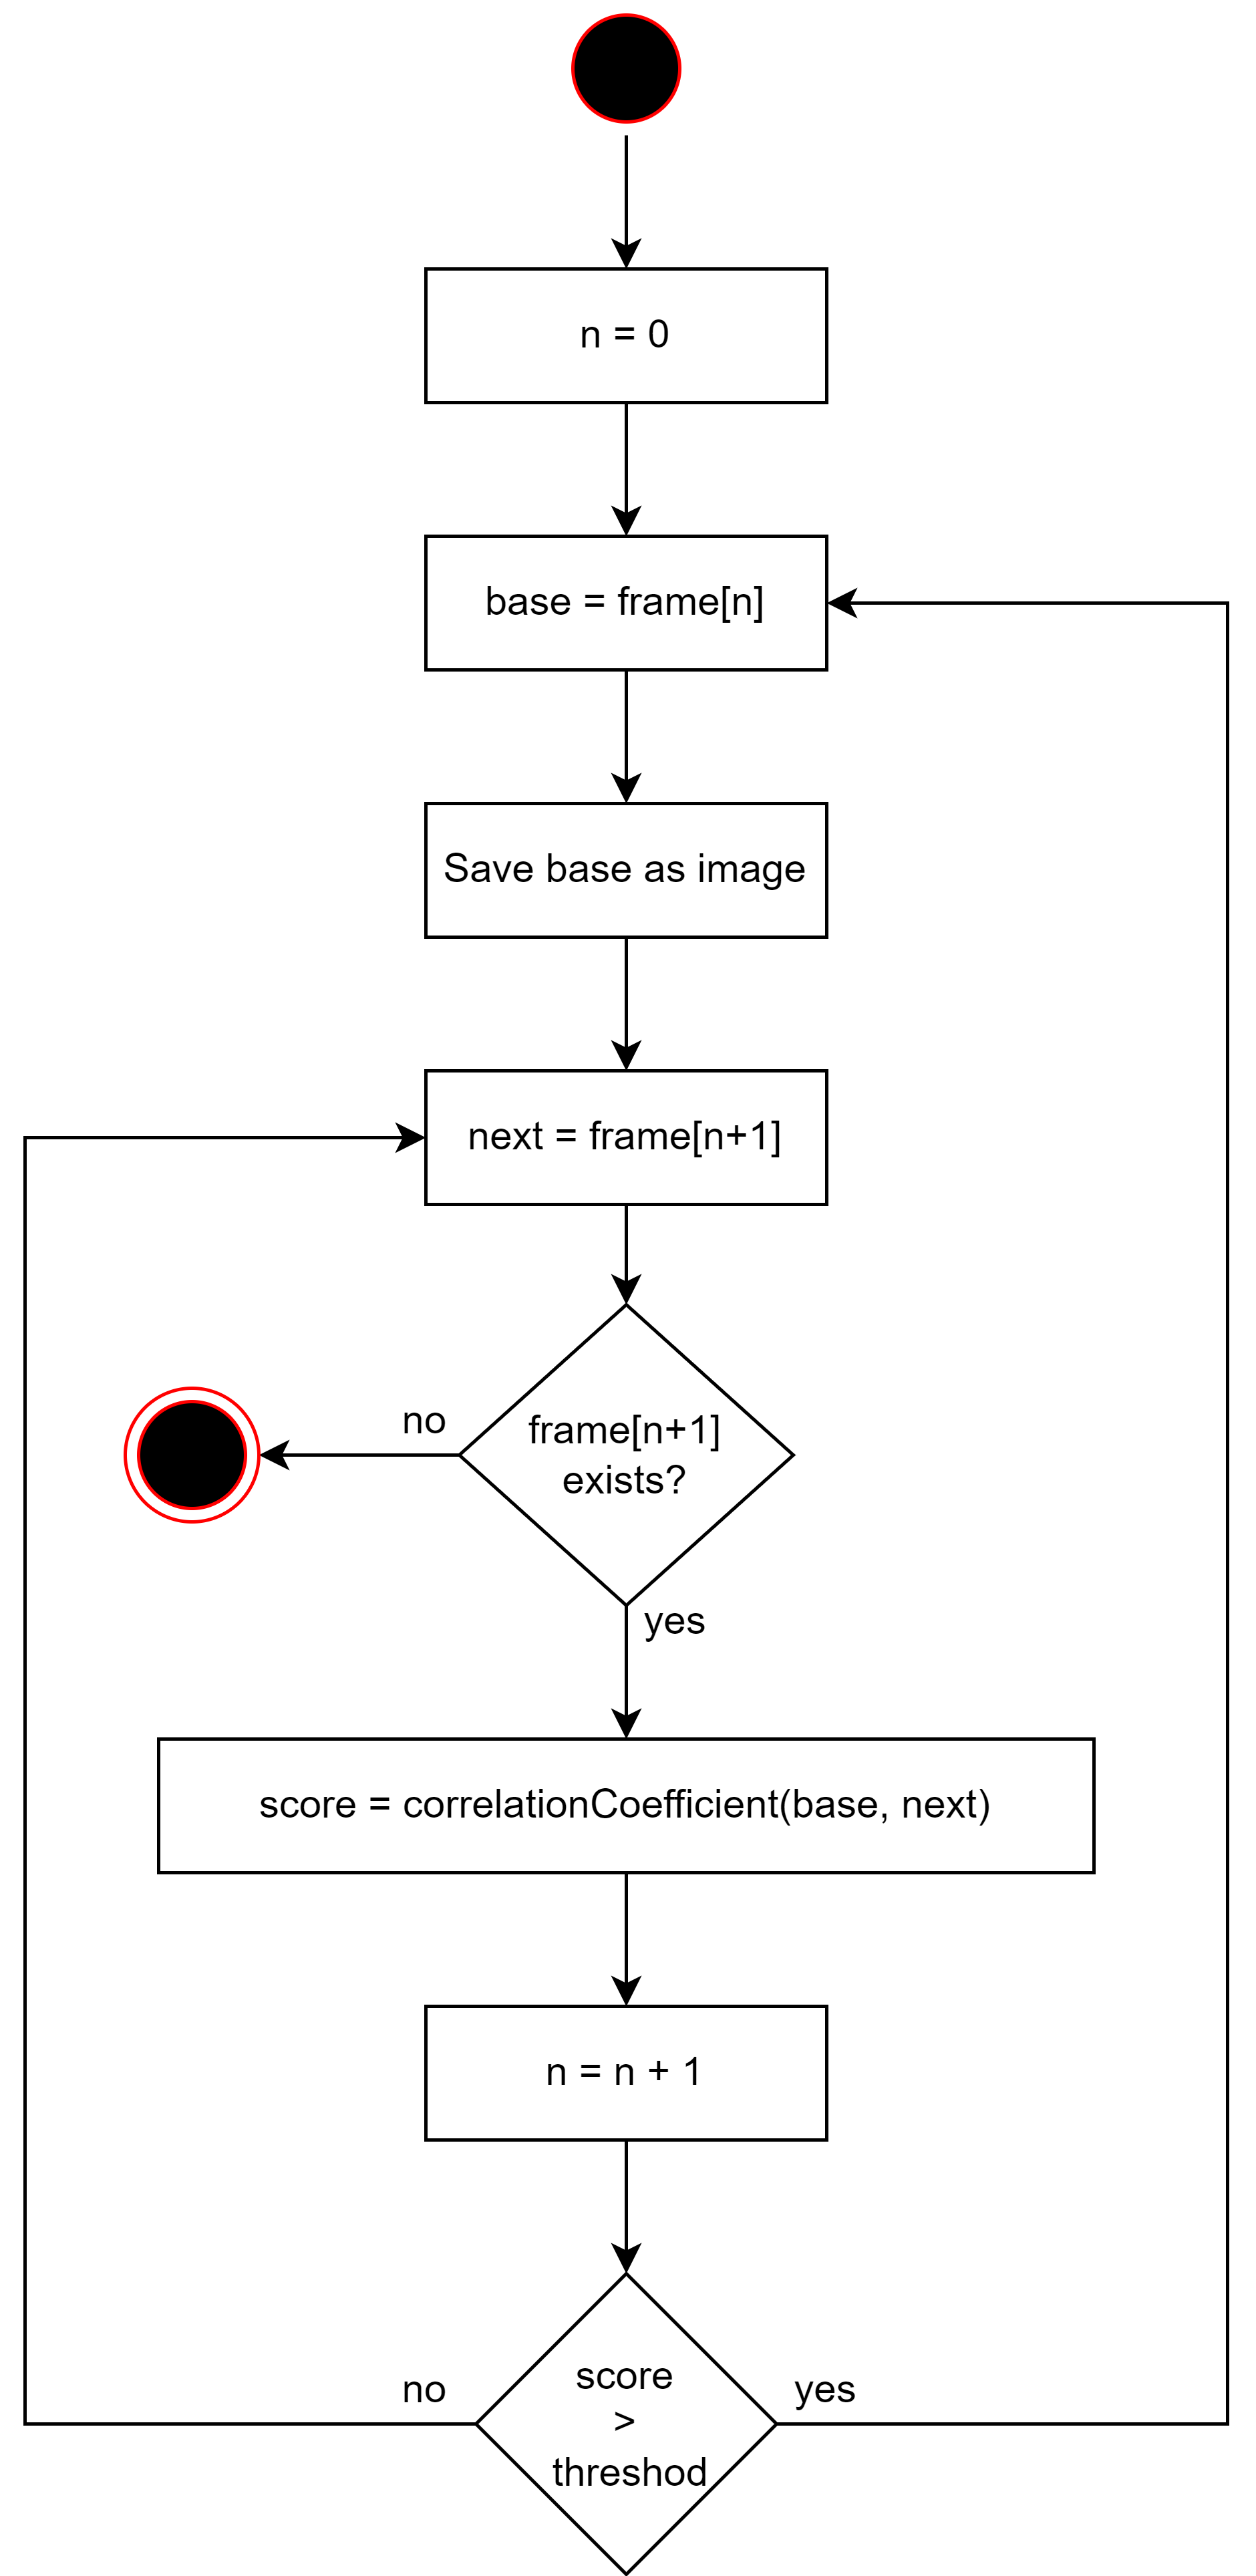
\includegraphics[width=0.5\textwidth]{diagrams/FlowChart-VideoToFrames.png}
    \caption{Video to frames flowchart}
    \end{figure}